% Created 2023-10-03 Tue 14:15
% Intended LaTeX compiler: pdflatex
\documentclass[11pt]{article}
\usepackage[utf8]{inputenc}
\usepackage[T1]{fontenc}
\usepackage{graphicx}
\usepackage{longtable}
\usepackage{wrapfig}
\usepackage{rotating}
\usepackage[normalem]{ulem}
\usepackage{amsmath}
\usepackage{amssymb}
\usepackage{capt-of}
\usepackage{hyperref}
\usepackage{siunitx, graphicx}
\graphicspath{ {./images/} }
\author{Hankertrix}
\date{\today}
\title{Rotation of Rigid Bodies Cheat Sheet}
\hypersetup{
 pdfauthor={Hankertrix},
 pdftitle={Rotation of Rigid Bodies Cheat Sheet},
 pdfkeywords={},
 pdfsubject={},
 pdfcreator={Emacs 29.1 (Org mode 9.6.6)}, 
 pdflang={English}}
\begin{document}

\maketitle
\setcounter{tocdepth}{2}
\tableofcontents

\newpage

\section{Definitions}
\label{sec:orge18b487}

\subsection{Tangential quantity}
\label{sec:org5943cf3}
In circular motion, a tangential quantity, like tangential velocity and tangential acceleration, refers to the quantity that is tangent to the circumference of the circle.

\subsection{Radial quantity}
\label{sec:orgf669a78}
In circular motion, a radial quantity, like radial velocity and radial acceleration, refers to the quantity that is perpendicular to the tangent of the circumference of the circle. That means that the quantity is either directed towards the centre of the circle, or directed outwards from the centre of the circle.

\subsection{Rotational analogue of Newton's Second Law}
\label{sec:org25c60f9}
The sum of torques, or the net torque, about a \textbf{fixed axis} is equal to the product of the moment of inertia (\(I\)) about the \textbf{same axis} and the angular acceleration (\(\alpha\)) about the \textbf{same axis}.
\\[0pt]

Essentially:
\[\sum \vec{\tau} = I \vec{\alpha}\]

Make sure that all quantities are calculated for the \textbf{same fixed axis}.
\\[0pt]

If an object is rotating with acceleration, as long as the axis the object is rotating about passes through its centre of mass (\(CM\)), we can still use the relation above, but with a stricter condition that \textbf{all quantities} are calculated \textbf{about the centre of mass}.
\[\sum \vec{\tau}_{CM} = I_{CM} \vec{\alpha}_{CM}\]

\newpage

\section{Formulas}
\label{sec:orga707c9b}

\subsection{Arc length (\(s\))}
\label{sec:org5bc164f}
\(s\) is the arc length or the tangential length, and it is given by:
\[s = r \theta, \ \theta \text{ in radians}\]

Where \(r\) is the radius of the circle that the object is rotating about.

\subsection{Angular displacement (\(\theta\))}
\label{sec:orgcaa1944}
\[\text{Angular displacement: } \theta = \frac{s}{r}\]

\subsection{Period (\(T\))}
\label{sec:org4eeaaaf}
The period is the time taken for an object to complete one full rotation, or spin a full circle.

\subsection{Frequency (\(f\))}
\label{sec:org12384b5}
\[\text{Frequency: } f = \frac{1}{T} \text{ where } T \text{ is the period}\]

\subsection{Angular velocity (\(\omega\))}
\label{sec:org52f6d96}
\begin{align*}
\text{Angular velocity: } \omega &= \frac{d \theta}{dt} \\
&= 2 \pi f \\
&= \frac{2 \pi}{T} \\
&= \frac{v_{tan}}{r}
\end{align*}

\subsection{Angular acceleration (\(\alpha\))}
\label{sec:org4dd2b18}
\[\text{Angular acceleration: } \alpha = \frac{d \omega}{dt}\]

\subsection{Comparing angular and linear quantities}
\label{sec:orga979e69}
The linear counterpart refers to the quantity in the tangential direction.

\begin{center}
\begin{tabular}{ c|c }
\(\textbf{Angular}\) & \(\textbf{Linear}\) \\
\hline
\(\theta\) & \(s = r\theta\) \\
\(\omega\) & \(v_{tan} = r\omega\) \\
\(\alpha\) & \(a_{tan} = r\alpha\) \\
\end{tabular}
\end{center}

For constant acceleration (both angular and linear), we have the following relations:
\begin{center}
\begin{tabular}{ c|c }
\(\textbf{Angular}\) & \(\textbf{Linear}\) \\
\hline
\(\omega_f = \omega_i + \alpha t\) & \(v_f = v_i + at\) \\
\(\theta - \theta_0 = \omega_i t + \frac{1}{2} \alpha t^2\) & \(x - x_0 = v_i + \frac{1}{2} a t^2\) \\
\(\omega_f^2 = \omega_i^2 + 2 \alpha(\theta - \theta_0)\) & \(v_f^2 = v_i^2 + 2a(x - x_0)\)
\end{tabular}
\end{center}

\subsection{Total linear acceleration}
\label{sec:org36f5c3b}
Total linear acceleration is given by:
\begin{align*}
\vec{a} &= \vec{a}_{tan} + \vec{a}_{radial} \\
&= \vec{a}_{tan} - \frac{(\vec{v}_{tan})^2}{R} \hat{r} \\
&= \vec{a}_{tan} - R \omega^2 \hat{r}
\end{align*}

\subsection{Torque (\(\vec{\tau}\)) (\(\unit{kg.m^2.s^{-2}}\))}
\label{sec:org5d5fcb0}
\[\vec{\tau} = \vec{r} \times \vec{F}\]

The magnitude of the torque is given by:
\[\tau = rF \sin \theta\]

\subsection{Moment of inertia (MOI)}
\label{sec:org29bc336}

\subsubsection{Discrete point masses}
\label{sec:org8ba25a9}
For a system of discrete point masses, the moment of inertia is:
\begin{align*}
I &= m_1 r_1^2 + m_2 r_2^2 + \cdots \\
&= \sum_{i} m_i r_i^2
\end{align*}

Where \(m\) is the masses of the particles that make up the body, and \(r\) is the \textbf{perpendicular distances} of the particles from the \textbf{rotation axis}.

\subsubsection{Continuous mass distribution}
\label{sec:orgda252fc}
For a system with continuous mass distribution, the moment of inertia is:
\begin{align*}
I &= \lim_{\Delta m_i \rightarrow 0} \sum_{i} \Delta m_i r_i^2 \\
&= \int r^2 \, dm
\end{align*}

\subsection{Parallel axis theorem}
\label{sec:orgae2c58a}
\[l_P = I_{CM} + Md^2\]

Where \(I_P\) refers to the moment of inertia about any other axis \textbf{parallel} to the axis through the object's centre of mass.

\subsection{Perpendicular axis theorem}
\label{sec:org71e7307}
The perpendicular axis theorem is \textbf{only applicable to flat (plane) objects}. It states that the sum of the moments of inertia of a plane object about \textbf{any two perpendicular} axes in the plane of the object, is \textbf{equal} to the moment of inertia about an axis through their point of intersection perpendicular to the plane of the object.
\\[0pt]

For example, if the flat object lies on the \(x - y\) plane, then:
\[I_z = I_x + I_y\]

\subsection{Rotational kinetic energy}
\label{sec:orgf326bf2}
\[K = \frac{1}{2} I \omega^2\]

Where \(I\) is the moment of inertia of the body about a given rotation axis, and \(\omega\) is the angular speed of the body.

\newpage

\subsection{Work-energy theorem for rotational motion}
\label{sec:org15c004c}
\begin{align*}
W &= \int \tau \, d \theta \\
&= \frac{1}{2} I \omega_f^2 - \frac{1}{2} I \omega_i^2
\end{align*}

Where \(\omega_f\) is the final angular velocity and \(\omega_i\) is the initial angular velocity. Essentially, the work down by the force is the change in kinetic energy of a rotating object.
\\[0pt]

The instantaneous power of the torque is:
\begin{align*}
P &= \frac{dW}{dt} \\
&= \tau \frac{d \theta}{dt} \\
&= \tau \omega
\end{align*}

\newpage


\section{Moment of inertia of common shapes}
\label{sec:orgb79aaed}
\[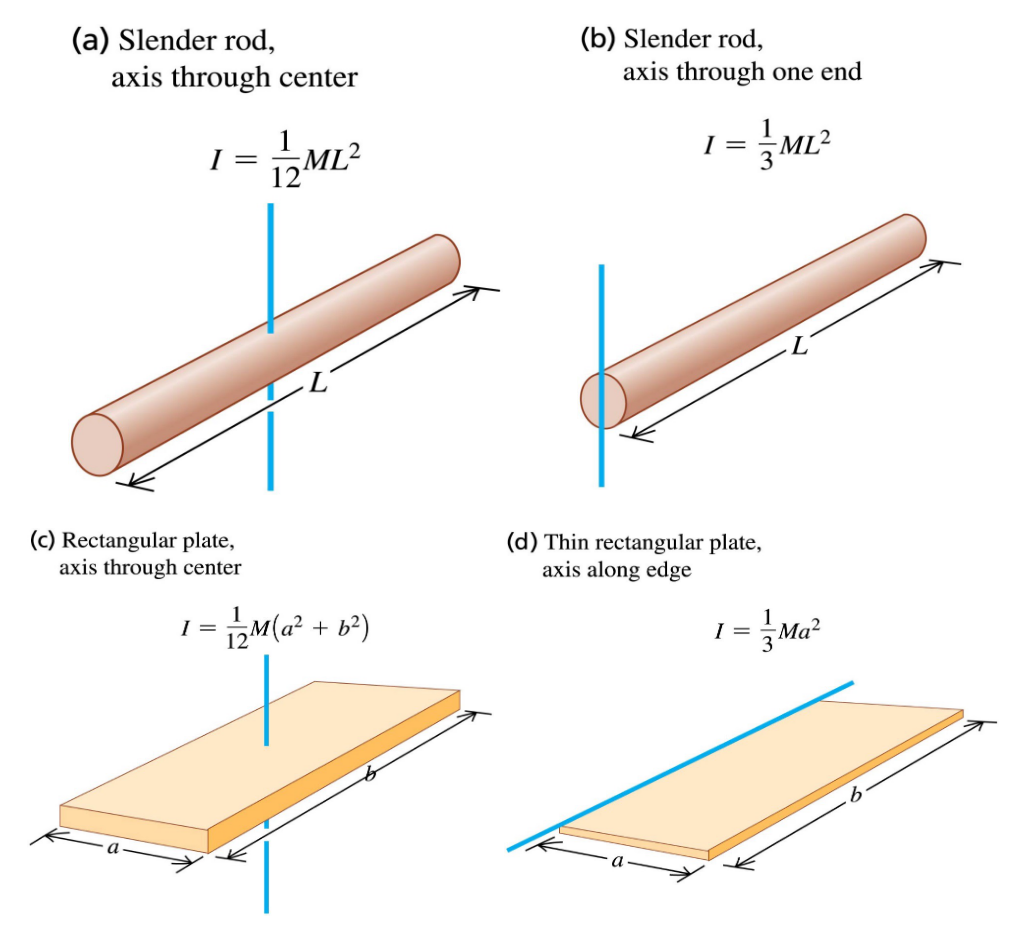
\includegraphics[width = \textwidth]{moments-of-inertia-1}\]

\[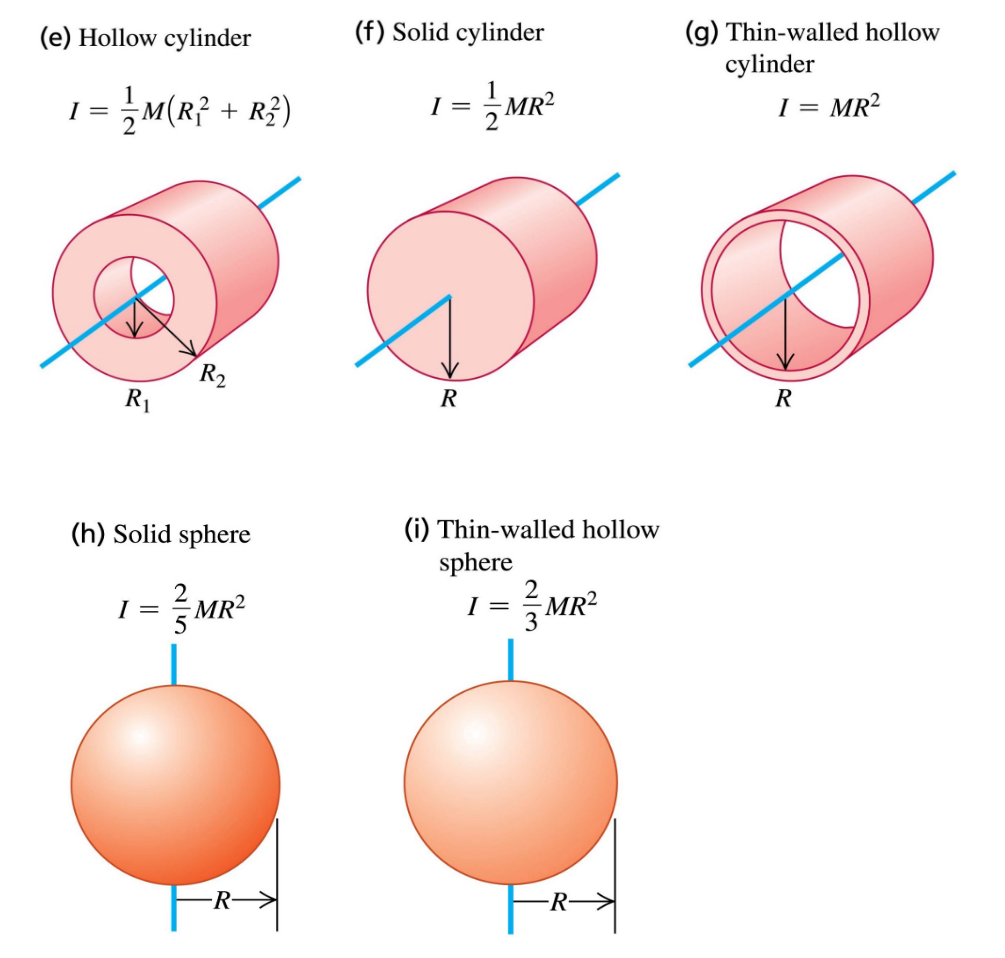
\includegraphics[width = \textwidth]{moments-of-inertia-2}\]

\newpage


\section{Rolling without slipping}
\label{sec:org9dc85fe}
When an object rolls without slipping, the length of the arc covered by the rotation in some duration is equal to the translational distance covered by the centre of mass, i.e.:
\begin{itemize}
\item Translational distance\(= v_{CM} \Delta t\)
\item Rotational arc length\(= R \omega \Delta t\)
\end{itemize}

Where \(\Delta t\) is the time interval during which the object is rolling. Thus:
\[v_{CM} = R \omega \text{ for rolling without slipping}\]

Note that \(v_{tan} = R \omega\) is always true, where \(v_{tan}\) is the tangential speed of a point on the circumference. Here, \(v_{CM}\) is the translational speed of the centre of mass and hence, \(v_{CM} = R \omega\) is only true for rolling without slipping.

\subsection{Kinetic energy}
\label{sec:org8759e52}

The total kinetic energy for an object that is rolling without slipping is the sum of the kinetic energy of pure rotation and the kinetic energy of pure translation, which is:
\[K_{total} = \frac{1}{2} I_{CM} \omega^2 + \frac{1}{2} mv_{CM}^2\]


\section{Differential quantities}
\label{sec:orgfb64e53}

\subsection{Cartesian coordinates}
\label{sec:org692ba87}

\[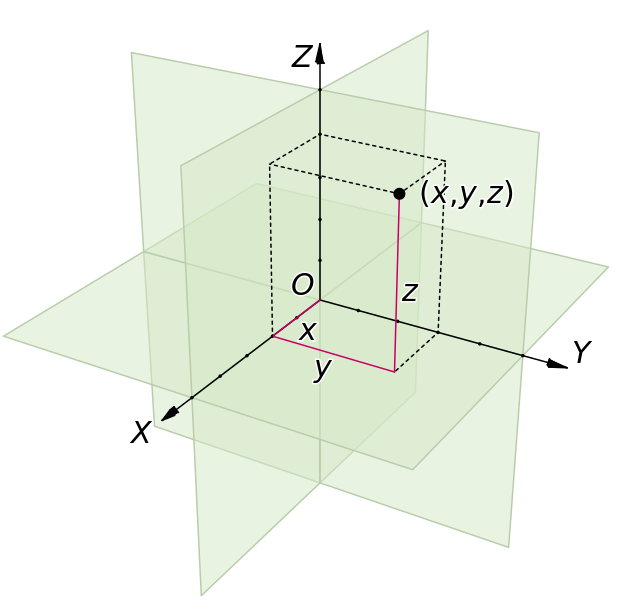
\includegraphics[scale = 0.4]{cartesian-coordinates}\]

Only the line and the volume elements below are generally applicable, as surface area elements depend on the surface specified in the question.

\subsubsection{Line element}
\label{sec:org4007592}
\[d \vec{l} = \hat{x} \, dx + \hat{y} \, dy + \hat{z} \, dz\]

\subsubsection{Surface area elements}
\label{sec:org87706c1}
\begin{itemize}
\item \(d \vec{s}_x = \hat{x} \, dy \, dz\)
\item \(d \vec{s}_y = \hat{y} \, dx \, dz\)
\item \(d \vec{s}_z = \hat{z} \, dx \, dy\)
\end{itemize}

\subsubsection{Volume element}
\label{sec:org161c2ed}
\[dV = dx \, dy \, dz\]

\subsection{Cylindrical coordinates}
\label{sec:orgc331cca}

\[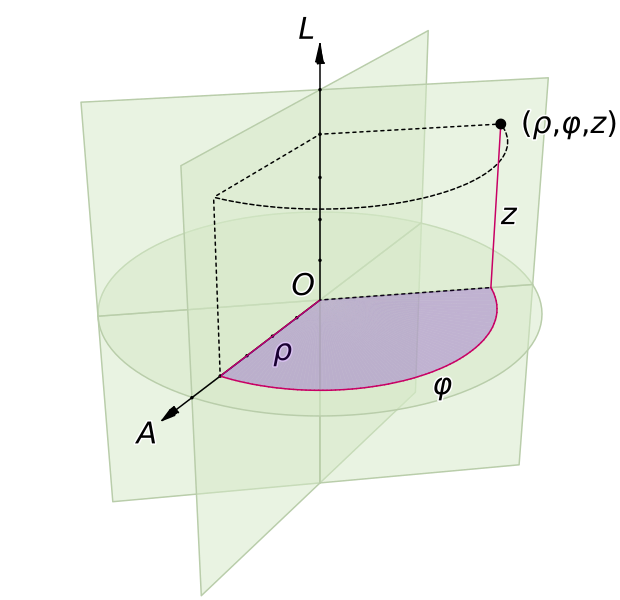
\includegraphics[scale = 0.4]{cylindrical-coordinates}\]

The radial distance on the \(x - y\) plane is given by the quantity \(s\) while most texts use either \(r\) or \(\rho\). We use \(r\) for a different radial distance in spherical coordinates and \(\rho\) to mean density.
\\[0pt]

\(\phi\) goes from \(0\) to \(2\pi\).

\[x = s \cos \phi\]
\[y = s \sin \phi\]
\[z = z\]

\subsubsection{Line element}
\label{sec:orge461887}
\[d \vec{l} = \hat{s} \, ds + \hat{\phi} (sd \phi) + \hat{z} \, dz\]

\subsubsection{Volume element}
\label{sec:org19bb775}
\[dV = s \, ds \, d \phi \, dz\]

\subsection{Spherical coordinates}
\label{sec:orgaeafab2}

\[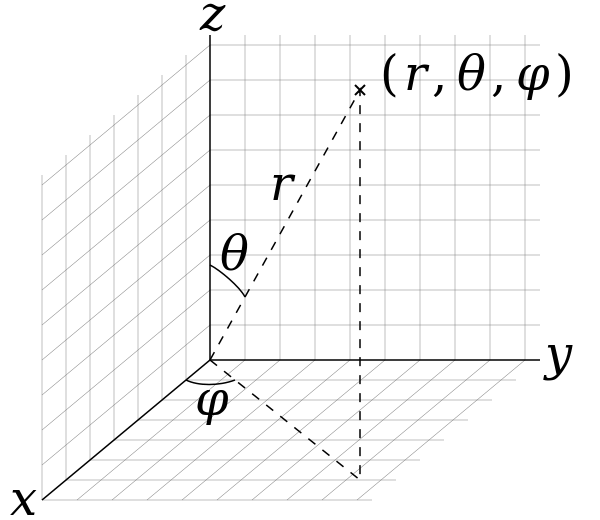
\includegraphics[width = \textwidth]{spherical-coordinates}\]

\(\phi\) goes from \(0\) to \(2\pi\) while \(\theta\) goes from \(0\) to \(\pi\).

\[x = r \sin \theta \cos \phi\]
\[y = r \sin \theta \sin \phi\]
\[z = r \cos \theta\]

\subsubsection{Line element}
\label{sec:orge8e8070}
\[d \vec{l} = \hat{r} \, dr + \hat{\phi} (r \sin \theta \, d \phi) + \hat{\theta} (r d \theta)\]

\subsubsection{Volume element}
\label{sec:org7cd8611}
\[dV = r^2 \sin \theta \, dr \, d \theta \, d \phi\]
\end{document}